\section{Deployment Architecture and Infrastructure}
\label{sec:deployment-architecture}

This section details the comprehensive deployment architecture for the Robotic Ultrasound System (RUS), covering infrastructure requirements, scalability considerations, and operational deployment strategies across diverse healthcare environments.

\subsection{System Deployment Models}

\subsubsection{Standalone Deployment}
The standalone deployment model is designed for smaller healthcare facilities or specialized clinics:

\begin{lstlisting}[language=C++, caption={Standalone Deployment Configuration}, label={lst:standalone-deployment}]
class StandaloneDeployment {
private:
    LocalComputeCluster compute_cluster_;
    LocalStorageSystem storage_system_;
    NetworkConfiguration network_config_;
    SecurityManager security_manager_;
    
public:
    bool initializeStandaloneSystem() {
        // Configure local compute resources
        compute_cluster_.configureNodes({
            {"primary_control", 16, 32}, // 16 cores, 32GB RAM
            {"image_processing", 32, 64}, // 32 cores, 64GB RAM
            {"safety_monitor", 8, 16}     // 8 cores, 16GB RAM
        });
        
        // Setup local storage with redundancy
        storage_system_.configureRAID({
            .raid_level = RAID10,
            .total_capacity = 10000, // 10TB
            .backup_strategy = AUTOMATED_INCREMENTAL
        });
        
        // Configure isolated network
        network_config_.setupIsolatedNetwork({
            .vlan_id = 100,
            .ip_range = "192.168.100.0/24",
            .encryption = WPA3_ENTERPRISE
        });
        
        return validateDeployment();
    }
    
    void configureFailoverSystems() {
        // Primary-backup configuration
        FailoverManager failover;
        failover.configurePrimaryBackup({
            .failover_threshold = std::chrono::seconds(5),
            .health_check_interval = std::chrono::seconds(1),
            .backup_sync_mode = SYNCHRONOUS
        });
    }
};
\end{lstlisting}

\subsubsection{Enterprise Deployment}
Large healthcare systems require scalable, distributed architectures:

\begin{figure}[htbp]
\centering
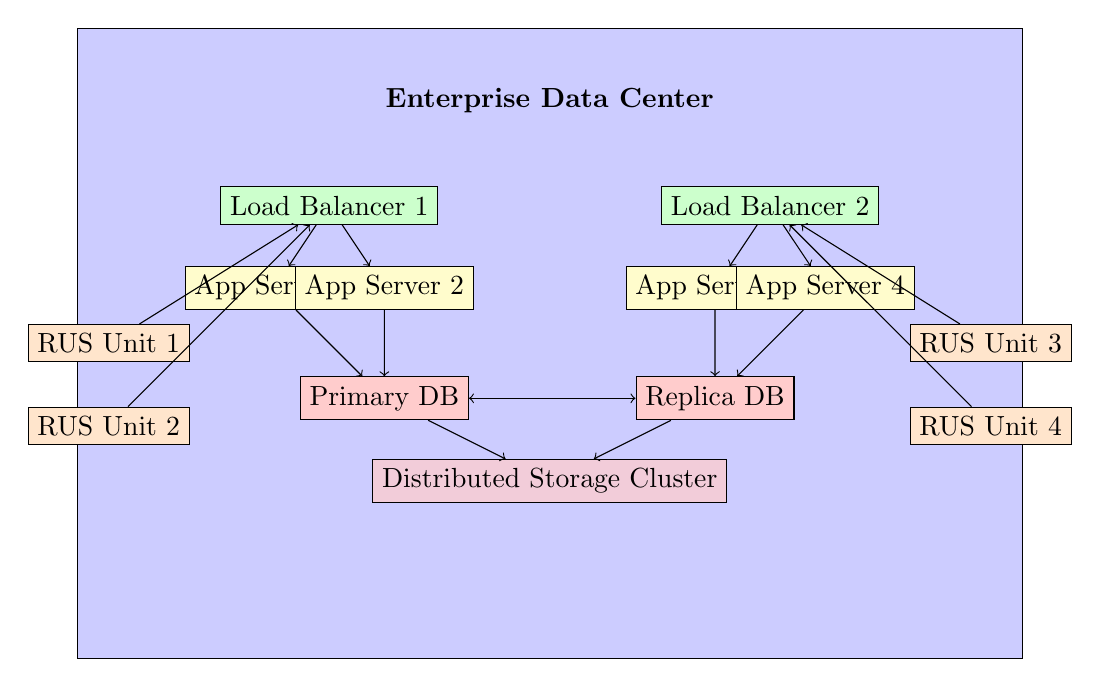
\begin{tikzpicture}[scale=0.7]
    % Data center architecture
    \node[draw, rectangle, fill=blue!20, minimum width=12cm, minimum height=8cm] (datacenter) at (0,0) {};
    \node[above] at (0,4) {\textbf{Enterprise Data Center}};
    
    % Load balancer tier
    \node[draw, rectangle, fill=green!20] (lb1) at (-4,2.5) {Load Balancer 1};
    \node[draw, rectangle, fill=green!20] (lb2) at (4,2.5) {Load Balancer 2};
    
    % Application tier
    \node[draw, rectangle, fill=yellow!20] (app1) at (-5,1) {App Server 1};
    \node[draw, rectangle, fill=yellow!20] (app2) at (-3,1) {App Server 2};
    \node[draw, rectangle, fill=yellow!20] (app3) at (3,1) {App Server 3};
    \node[draw, rectangle, fill=yellow!20] (app4) at (5,1) {App Server 4};
    
    % Database tier
    \node[draw, rectangle, fill=red!20] (db1) at (-3,-1) {Primary DB};
    \node[draw, rectangle, fill=red!20] (db2) at (3,-1) {Replica DB};
    
    % Storage tier
    \node[draw, rectangle, fill=purple!20] (storage) at (0,-2.5) {Distributed Storage Cluster};
    
    % Connections
    \draw[->] (lb1) -- (app1);
    \draw[->] (lb1) -- (app2);
    \draw[->] (lb2) -- (app3);
    \draw[->] (lb2) -- (app4);
    
    \draw[->] (app1) -- (db1);
    \draw[->] (app2) -- (db1);
    \draw[->] (app3) -- (db2);
    \draw[->] (app4) -- (db2);
    
    \draw[<->] (db1) -- (db2);
    \draw[->] (db1) -- (storage);
    \draw[->] (db2) -- (storage);
    
    % External connections
    \node[draw, rectangle, fill=orange!20] (rus1) at (-8,0) {RUS Unit 1};
    \node[draw, rectangle, fill=orange!20] (rus2) at (-8,-1.5) {RUS Unit 2};
    \node[draw, rectangle, fill=orange!20] (rus3) at (8,0) {RUS Unit 3};
    \node[draw, rectangle, fill=orange!20] (rus4) at (8,-1.5) {RUS Unit 4};
    
    \draw[->] (rus1) -- (lb1);
    \draw[->] (rus2) -- (lb1);
    \draw[->] (rus3) -- (lb2);
    \draw[->] (rus4) -- (lb2);
    
\end{tikzpicture}
\caption{Enterprise Deployment Architecture}
\label{fig:enterprise-deployment}
\end{figure}

\subsubsection{Cloud-Hybrid Deployment}
Modern deployments leverage cloud infrastructure for scalability and cost optimization:

\begin{lstlisting}[language=Python, caption={Cloud-Hybrid Infrastructure Management}, label={lst:cloud-hybrid}]
class CloudHybridDeployment:
    def __init__(self):
        self.local_infrastructure = LocalInfrastructure()
        self.cloud_provider = CloudProvider("AWS")  # or Azure, GCP
        self.edge_nodes = []
        
    def deploy_hybrid_architecture(self):
        # Local edge processing for real-time requirements
        edge_config = {
            'compute_nodes': 4,
            'gpu_acceleration': True,
            'storage_tier': 'NVMe_SSD',
            'network_latency_max': '1ms'
        }
        
        local_edge = self.local_infrastructure.deploy_edge_cluster(edge_config)
        
        # Cloud backend for analytics and storage
        cloud_config = {
            'instance_types': ['c5.4xlarge', 'r5.8xlarge'],
            'auto_scaling': {
                'min_instances': 2,
                'max_instances': 20,
                'target_cpu_utilization': 70
            },
            'storage': {
                'type': 'S3',
                'tier': 'Standard-IA',
                'encryption': 'AES-256'
            }
        }
        
        cloud_backend = self.cloud_provider.deploy_backend(cloud_config)
        
        # Configure secure connectivity
        self.setup_vpn_connection(local_edge, cloud_backend)
        
        return {
            'edge_cluster': local_edge,
            'cloud_backend': cloud_backend,
            'total_capacity': self.calculate_total_capacity()
        }
    
    def setup_data_flow_pipeline(self):
        # Real-time data processing at edge
        edge_pipeline = DataPipeline([
            RealTimeImageProcessor(),
            SafetyMonitor(),
            LocalAnalytics()
        ])
        
        # Batch processing in cloud
        cloud_pipeline = DataPipeline([
            BatchImageAnalyzer(),
            MachineLearningTrainer(),
            LongTermStorage(),
            ComplianceReporting()
        ])
        
        # Configure data synchronization
        sync_manager = DataSyncManager(
            edge_retention_days=30,
            cloud_retention_years=7,
            sync_schedule='0 2 * * *'  # Daily at 2 AM
        )
        
        return {
            'edge_pipeline': edge_pipeline,
            'cloud_pipeline': cloud_pipeline,
            'sync_manager': sync_manager
        }
\end{lstlisting}

\subsection{Infrastructure Requirements}

\subsubsection{Compute Requirements}
The RUS system requires substantial computational resources for real-time processing:

\begin{table}[htbp]
\centering
\caption{Compute Resource Requirements}
\label{tab:compute-requirements}
\begin{tabular}{|l|c|c|c|c|}
\hline
\textbf{Component} & \textbf{CPU Cores} & \textbf{RAM (GB)} & \textbf{GPU} & \textbf{Latency Req.} \\
\hline
Real-time Control & 8-16 & 32 & Optional & $< 1$ ms \\
Image Processing & 16-32 & 64-128 & NVIDIA RTX 4090 & $< 10$ ms \\
Path Planning & 8-16 & 32-64 & Optional & $< 100$ ms \\
Safety Systems & 4-8 & 16 & None & $< 1$ ms \\
Analytics Engine & 8-32 & 64-256 & NVIDIA A100 & $< 1$ s \\
\hline
\textbf{Total Minimum} & \textbf{44} & \textbf{208} & \textbf{2 GPUs} & - \\
\textbf{Recommended} & \textbf{80} & \textbf{512} & \textbf{4 GPUs} & - \\
\hline
\end{tabular}
\end{table}

\subsubsection{Storage Architecture}
A tiered storage strategy optimizes performance and cost:

\begin{lstlisting}[language=C++, caption={Tiered Storage Manager}, label={lst:tiered-storage}]
class TieredStorageManager {
private:
    enum StorageTier {
        HOT_TIER,      // NVMe SSD - Active data
        WARM_TIER,     // SATA SSD - Recent data
        COLD_TIER,     // HDD - Archive data
        GLACIER_TIER   // Cloud - Long-term archive
    };
    
    struct StoragePolicy {
        std::chrono::hours hot_retention{24};
        std::chrono::days warm_retention{30};
        std::chrono::days cold_retention{365};
        std::chrono::years glacier_retention{7};
    };
    
    StoragePolicy policy_;
    std::map<StorageTier, std::unique_ptr<StorageBackend>> backends_;
    
public:
    void configureStorageTiers() {
        // Hot tier - NVMe for active procedures
        backends_[HOT_TIER] = std::make_unique<NVMeBackend>(
            StorageConfig{
                .capacity_gb = 2000,
                .raid_level = RAID10,
                .encryption = true,
                .compression = false
            }
        );
        
        // Warm tier - SSD for recent procedures
        backends_[WARM_TIER] = std::make_unique<SSDBackend>(
            StorageConfig{
                .capacity_gb = 20000,
                .raid_level = RAID5,
                .encryption = true,
                .compression = true
            }
        );
        
        // Cold tier - HDD for archive
        backends_[COLD_TIER] = std::make_unique<HDDBackend>(
            StorageConfig{
                .capacity_gb = 100000,
                .raid_level = RAID6,
                .encryption = true,
                .compression = true
            }
        );
        
        // Glacier tier - Cloud for compliance
        backends_[GLACIER_TIER] = std::make_unique<CloudBackend>(
            CloudConfig{
                .provider = "AWS_GLACIER",
                .encryption = "AES_256",
                .geo_replication = true
            }
        );
    }
    
    void manageDataLifecycle(const DataObject& data) {
        auto age = std::chrono::system_clock::now() - data.creation_time;
        
        if (age > policy_.glacier_retention) {
            // Consider deletion based on retention policy
            evaluateRetentionPolicy(data);
        } else if (age > policy_.cold_retention) {
            migrateToTier(data, GLACIER_TIER);
        } else if (age > policy_.warm_retention) {
            migrateToTier(data, COLD_TIER);
        } else if (age > policy_.hot_retention) {
            migrateToTier(data, WARM_TIER);
        }
    }
};
\end{lstlisting}

\subsection{Network Architecture and Security}

\subsubsection{Network Topology Design}
The network architecture prioritizes security, performance, and reliability:

\begin{figure}[htbp]
\centering
\begin{tikzpicture}[scale=0.8]
    % Network layers
    \node[draw, rectangle, fill=red!20, minimum width=10cm, minimum height=1.5cm] (dmz) at (0,4) {};
    \node[above] at (0,4.75) {\textbf{DMZ - Demilitarized Zone}};
    
    \node[draw, rectangle, fill=yellow!20, minimum width=10cm, minimum height=1.5cm] (clinical) at (0,2) {};
    \node[above] at (0,2.75) {\textbf{Clinical Network}};
    
    \node[draw, rectangle, fill=green!20, minimum width=10cm, minimum height=1.5cm] (device) at (0,0) {};
    \node[above] at (0,0.75) {\textbf{Device Network}};
    
    \node[draw, rectangle, fill=blue!20, minimum width=10cm, minimum height=1.5cm] (management) at (0,-2) {};
    \node[above] at (0,-1.25) {\textbf{Management Network}};
    
    % Firewalls
    \node[draw, diamond, fill=orange!30] (fw1) at (-3,3) {FW};
    \node[draw, diamond, fill=orange!30] (fw2) at (3,3) {FW};
    \node[draw, diamond, fill=orange!30] (fw3) at (-3,1) {FW};
    \node[draw, diamond, fill=orange!30] (fw4) at (3,1) {FW};
    \node[draw, diamond, fill=orange!30] (fw5) at (0,-1) {FW};
    
    % Network components in each zone
    \node at (-3,4) {Web Portal};
    \node at (0,4) {API Gateway};
    \node at (3,4) {Load Balancer};
    
    \node at (-3,2) {EMR Integration};
    \node at (0,2) {Clinical Apps};
    \node at (3,2) {PACS Server};
    
    \node at (-3,0) {RUS Controller};
    \node at (0,0) {Sensor Network};
    \node at (3,0) {Robot Arm};
    
    \node at (-2,-2) {Monitoring};
    \node at (0,-2) {Backup Systems};
    \node at (2,-2) {Admin Console};
    
\end{tikzpicture}
\caption{Segmented Network Architecture}
\label{fig:network-architecture}
\end{figure}

\subsubsection{Security Implementation}
Comprehensive security measures protect sensitive medical data:

\begin{lstlisting}[language=C++, caption={Network Security Manager}, label={lst:network-security}]
class NetworkSecurityManager {
private:
    FirewallManager firewall_;
    IntrusionDetectionSystem ids_;
    VPNManager vpn_;
    CertificateManager certificates_;
    
public:
    void initializeSecurityInfrastructure() {
        // Configure network segmentation
        firewall_.createSecurityZones({
            {"DMZ", "192.168.10.0/24", SecurityLevel::MEDIUM},
            {"CLINICAL", "192.168.20.0/24", SecurityLevel::HIGH},
            {"DEVICE", "192.168.30.0/24", SecurityLevel::CRITICAL},
            {"MGMT", "192.168.40.0/24", SecurityLevel::HIGH}
        });
        
        // Setup intrusion detection
        ids_.configureRules({
            {"MEDICAL_DEVICE_ANOMALY", "Unusual device communication patterns"},
            {"DATA_EXFILTRATION", "Large data transfers to external networks"},
            {"PRIVILEGE_ESCALATION", "Unauthorized administrative access attempts"},
            {"PROTOCOL_VIOLATION", "Non-standard medical device protocols"}
        });
        
        // Configure VPN for remote access
        vpn_.setupClientCertificateAuth({
            .certificate_authority = "InternalCA",
            .key_length = 4096,
            .encryption_algorithm = "AES-256-GCM",
            .perfect_forward_secrecy = true
        });
    }
    
    void monitorSecurityEvents() {
        auto events = ids_.getRecentEvents();
        
        for (const auto& event : events) {
            switch (event.severity) {
                case SecuritySeverity::CRITICAL:
                    handleCriticalSecurityEvent(event);
                    break;
                case SecuritySeverity::HIGH:
                    escalateToSecurityTeam(event);
                    break;
                case SecuritySeverity::MEDIUM:
                    logSecurityEvent(event);
                    break;
                case SecuritySeverity::LOW:
                    updateSecurityDashboard(event);
                    break;
            }
        }
    }
    
private:
    void handleCriticalSecurityEvent(const SecurityEvent& event) {
        // Immediate response protocol
        if (event.type == "DEVICE_COMPROMISE") {
            // Isolate affected device network segment
            firewall_.isolateSegment(event.source_network);
            
            // Alert incident response team
            incident_response_.triggerEmergencyResponse(event);
            
            // Preserve forensic evidence
            forensics_.captureNetworkState(event.timestamp);
        }
    }
};
\end{lstlisting}

\subsection{Scalability and Performance Optimization}

\subsubsection{Horizontal Scaling Architecture}
The system supports dynamic scaling based on demand:

\begin{table}[htbp]
\centering
\caption{Scaling Metrics and Thresholds}
\label{tab:scaling-metrics}
\begin{tabular}{|l|c|c|c|}
\hline
\textbf{Metric} & \textbf{Scale Up} & \textbf{Scale Down} & \textbf{Response Time} \\
\hline
CPU Utilization & $> 75\%$ & $< 30\%$ & 2 minutes \\
Memory Usage & $> 80\%$ & $< 40\%$ & 1 minute \\
Network Latency & $> 50$ ms & $< 10$ ms & 30 seconds \\
Queue Depth & $> 100$ & $< 10$ & 1 minute \\
Active Sessions & $> 80\%$ capacity & $< 40\%$ capacity & 2 minutes \\
\hline
\end{tabular}
\end{table}

\subsubsection{Performance Monitoring and Optimization}

\begin{lstlisting}[language=Python, caption={Performance Monitoring System}, label={lst:performance-monitoring}]
class PerformanceMonitoringSystem:
    def __init__(self):
        self.metrics_collector = MetricsCollector()
        self.alerting_system = AlertingSystem()
        self.auto_scaler = AutoScaler()
        
    def monitor_system_performance(self):
        metrics = self.metrics_collector.collect_metrics()
        
        # Analyze performance trends
        performance_analysis = self.analyze_performance_trends(metrics)
        
        # Check for performance degradation
        if performance_analysis.degradation_detected:
            self.handle_performance_degradation(performance_analysis)
        
        # Optimize resource allocation
        optimization_recommendations = self.generate_optimization_recommendations(metrics)
        
        if optimization_recommendations.auto_apply:
            self.apply_optimizations(optimization_recommendations)
        
        return {
            'current_metrics': metrics,
            'performance_analysis': performance_analysis,
            'optimizations': optimization_recommendations
        }
    
    def analyze_performance_trends(self, metrics):
        # Implement trend analysis
        cpu_trend = self.calculate_trend(metrics.cpu_history)
        memory_trend = self.calculate_trend(metrics.memory_history)
        latency_trend = self.calculate_trend(metrics.latency_history)
        
        # Predict future performance
        future_load = self.predict_load(metrics.historical_patterns)
        
        # Detect anomalies
        anomalies = self.detect_anomalies(metrics)
        
        return PerformanceAnalysis(
            cpu_trend=cpu_trend,
            memory_trend=memory_trend,
            latency_trend=latency_trend,
            predicted_load=future_load,
            anomalies=anomalies,
            degradation_detected=len(anomalies) > 0
        )
    
    def generate_optimization_recommendations(self, metrics):
        recommendations = []
        
        # CPU optimization
        if metrics.cpu_utilization > 0.8:
            recommendations.append(OptimizationAction(
                type='SCALE_UP_CPU',
                priority='HIGH',
                estimated_impact='20% latency reduction'
            ))
        
        # Memory optimization
        if metrics.memory_fragmentation > 0.3:
            recommendations.append(OptimizationAction(
                type='MEMORY_DEFRAGMENTATION',
                priority='MEDIUM',
                estimated_impact='15% memory efficiency improvement'
            ))
        
        # Network optimization
        if metrics.network_congestion > 0.6:
            recommendations.append(OptimizationAction(
                type='TRAFFIC_SHAPING',
                priority='HIGH',
                estimated_impact='30% latency reduction'
            ))
        
        return OptimizationRecommendations(
            actions=recommendations,
            auto_apply=all(action.priority != 'CRITICAL' for action in recommendations)
        )
\end{lstlisting}

\subsection{Disaster Recovery and Business Continuity}

\subsubsection{Backup and Recovery Strategy}
A comprehensive backup strategy ensures data protection and system availability:

\begin{figure}[htbp]
\centering
\begin{tikzpicture}[scale=0.8]
    % Backup tiers
    \node[draw, rectangle, fill=green!20, align=center] (local) at (0,3) {Local Backup\\(Daily)};
    \node[draw, rectangle, fill=blue!20, align=center] (regional) at (0,1.5) {Regional Backup\\(Weekly)};
    \node[draw, rectangle, fill=purple!20, align=center] (cloud) at (0,0) {Cloud Backup\\(Monthly)};
    
    % Recovery times
    \node[right=2cm of local] {RTO: 15 minutes};
    \node[right=2cm of regional] {RTO: 2 hours};
    \node[right=2cm of cloud] {RTO: 24 hours};
    
    % Data flow
    \node[left=2cm of local] (primary) {Primary System};
    \draw[->] (primary) -- (local);
    \draw[->] (local) -- (regional);
    \draw[->] (regional) -- (cloud);
    
    % Backup frequency
    \node[left=1cm of local] {\footnotesize 24/7};
    \node[left=1cm of regional] {\footnotesize Weekly};
    \node[left=1cm of cloud] {\footnotesize Monthly};
    
\end{tikzpicture}
\caption{Multi-Tier Backup and Recovery Architecture}
\label{fig:backup-architecture}
\end{figure}

This deployment architecture ensures that the RUS system can be successfully implemented across diverse healthcare environments while maintaining high performance, security, and reliability standards. The modular design allows for flexible deployment options that can scale from small clinics to large hospital networks.
